% Options for packages loaded elsewhere
\PassOptionsToPackage{unicode}{hyperref}
\PassOptionsToPackage{hyphens}{url}
%
\documentclass[
]{article}
\usepackage{lmodern}
\usepackage{amssymb,amsmath}
\usepackage{ifxetex,ifluatex}
\ifnum 0\ifxetex 1\fi\ifluatex 1\fi=0 % if pdftex
  \usepackage[T1]{fontenc}
  \usepackage[utf8]{inputenc}
  \usepackage{textcomp} % provide euro and other symbols
\else % if luatex or xetex
  \usepackage{unicode-math}
  \defaultfontfeatures{Scale=MatchLowercase}
  \defaultfontfeatures[\rmfamily]{Ligatures=TeX,Scale=1}
\fi
% Use upquote if available, for straight quotes in verbatim environments
\IfFileExists{upquote.sty}{\usepackage{upquote}}{}
\IfFileExists{microtype.sty}{% use microtype if available
  \usepackage[]{microtype}
  \UseMicrotypeSet[protrusion]{basicmath} % disable protrusion for tt fonts
}{}
\makeatletter
\@ifundefined{KOMAClassName}{% if non-KOMA class
  \IfFileExists{parskip.sty}{%
    \usepackage{parskip}
  }{% else
    \setlength{\parindent}{0pt}
    \setlength{\parskip}{6pt plus 2pt minus 1pt}}
}{% if KOMA class
  \KOMAoptions{parskip=half}}
\makeatother
\usepackage{xcolor}
\IfFileExists{xurl.sty}{\usepackage{xurl}}{} % add URL line breaks if available
\IfFileExists{bookmark.sty}{\usepackage{bookmark}}{\usepackage{hyperref}}
\hypersetup{
  pdftitle={Diffusion},
  hidelinks,
  pdfcreator={LaTeX via pandoc}}
\urlstyle{same} % disable monospaced font for URLs
\usepackage[margin=1in]{geometry}
\usepackage{color}
\usepackage{fancyvrb}
\newcommand{\VerbBar}{|}
\newcommand{\VERB}{\Verb[commandchars=\\\{\}]}
\DefineVerbatimEnvironment{Highlighting}{Verbatim}{commandchars=\\\{\}}
% Add ',fontsize=\small' for more characters per line
\usepackage{framed}
\definecolor{shadecolor}{RGB}{248,248,248}
\newenvironment{Shaded}{\begin{snugshade}}{\end{snugshade}}
\newcommand{\AlertTok}[1]{\textcolor[rgb]{0.94,0.16,0.16}{#1}}
\newcommand{\AnnotationTok}[1]{\textcolor[rgb]{0.56,0.35,0.01}{\textbf{\textit{#1}}}}
\newcommand{\AttributeTok}[1]{\textcolor[rgb]{0.77,0.63,0.00}{#1}}
\newcommand{\BaseNTok}[1]{\textcolor[rgb]{0.00,0.00,0.81}{#1}}
\newcommand{\BuiltInTok}[1]{#1}
\newcommand{\CharTok}[1]{\textcolor[rgb]{0.31,0.60,0.02}{#1}}
\newcommand{\CommentTok}[1]{\textcolor[rgb]{0.56,0.35,0.01}{\textit{#1}}}
\newcommand{\CommentVarTok}[1]{\textcolor[rgb]{0.56,0.35,0.01}{\textbf{\textit{#1}}}}
\newcommand{\ConstantTok}[1]{\textcolor[rgb]{0.00,0.00,0.00}{#1}}
\newcommand{\ControlFlowTok}[1]{\textcolor[rgb]{0.13,0.29,0.53}{\textbf{#1}}}
\newcommand{\DataTypeTok}[1]{\textcolor[rgb]{0.13,0.29,0.53}{#1}}
\newcommand{\DecValTok}[1]{\textcolor[rgb]{0.00,0.00,0.81}{#1}}
\newcommand{\DocumentationTok}[1]{\textcolor[rgb]{0.56,0.35,0.01}{\textbf{\textit{#1}}}}
\newcommand{\ErrorTok}[1]{\textcolor[rgb]{0.64,0.00,0.00}{\textbf{#1}}}
\newcommand{\ExtensionTok}[1]{#1}
\newcommand{\FloatTok}[1]{\textcolor[rgb]{0.00,0.00,0.81}{#1}}
\newcommand{\FunctionTok}[1]{\textcolor[rgb]{0.00,0.00,0.00}{#1}}
\newcommand{\ImportTok}[1]{#1}
\newcommand{\InformationTok}[1]{\textcolor[rgb]{0.56,0.35,0.01}{\textbf{\textit{#1}}}}
\newcommand{\KeywordTok}[1]{\textcolor[rgb]{0.13,0.29,0.53}{\textbf{#1}}}
\newcommand{\NormalTok}[1]{#1}
\newcommand{\OperatorTok}[1]{\textcolor[rgb]{0.81,0.36,0.00}{\textbf{#1}}}
\newcommand{\OtherTok}[1]{\textcolor[rgb]{0.56,0.35,0.01}{#1}}
\newcommand{\PreprocessorTok}[1]{\textcolor[rgb]{0.56,0.35,0.01}{\textit{#1}}}
\newcommand{\RegionMarkerTok}[1]{#1}
\newcommand{\SpecialCharTok}[1]{\textcolor[rgb]{0.00,0.00,0.00}{#1}}
\newcommand{\SpecialStringTok}[1]{\textcolor[rgb]{0.31,0.60,0.02}{#1}}
\newcommand{\StringTok}[1]{\textcolor[rgb]{0.31,0.60,0.02}{#1}}
\newcommand{\VariableTok}[1]{\textcolor[rgb]{0.00,0.00,0.00}{#1}}
\newcommand{\VerbatimStringTok}[1]{\textcolor[rgb]{0.31,0.60,0.02}{#1}}
\newcommand{\WarningTok}[1]{\textcolor[rgb]{0.56,0.35,0.01}{\textbf{\textit{#1}}}}
\usepackage{graphicx,grffile}
\makeatletter
\def\maxwidth{\ifdim\Gin@nat@width>\linewidth\linewidth\else\Gin@nat@width\fi}
\def\maxheight{\ifdim\Gin@nat@height>\textheight\textheight\else\Gin@nat@height\fi}
\makeatother
% Scale images if necessary, so that they will not overflow the page
% margins by default, and it is still possible to overwrite the defaults
% using explicit options in \includegraphics[width, height, ...]{}
\setkeys{Gin}{width=\maxwidth,height=\maxheight,keepaspectratio}
% Set default figure placement to htbp
\makeatletter
\def\fps@figure{htbp}
\makeatother
\setlength{\emergencystretch}{3em} % prevent overfull lines
\providecommand{\tightlist}{%
  \setlength{\itemsep}{0pt}\setlength{\parskip}{0pt}}
\setcounter{secnumdepth}{-\maxdimen} % remove section numbering

\title{Diffusion}
\author{}
\date{\vspace{-2.5em}}

\begin{document}
\maketitle

\hypertarget{diffusion}{%
\subsection{Diffusion}\label{diffusion}}

Diffusion can be implemented as a partial differential equation
Complicated to solve - but there are tool in R for specific types of
partial differential equations
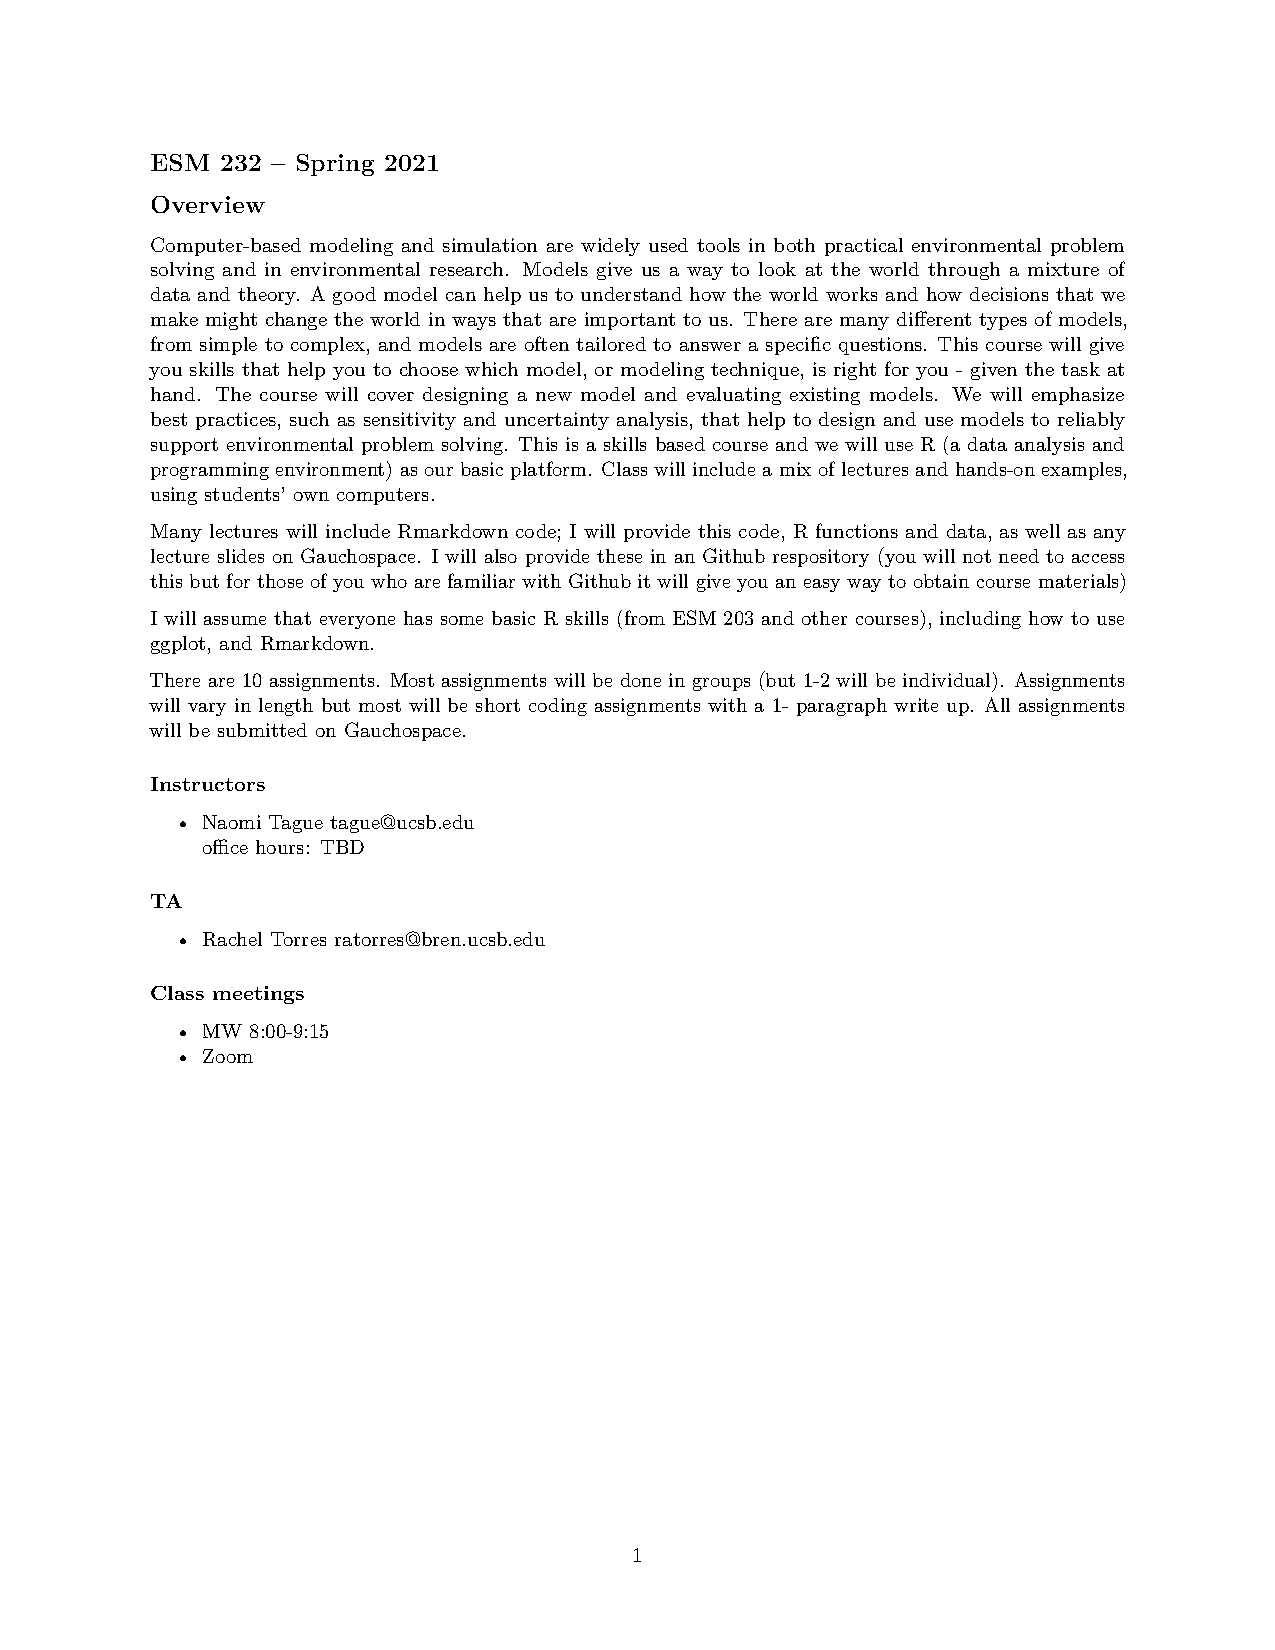
\includegraphics{https://cran.r-project.org/web/packages/ReacTran/index.html}

More info on differential equations in R
\includegraphics{http://www-labs.iro.umontreal.ca/~mignotte/IFT2425/Documents/Solving_Differential_Equations_In_R_Soetaert_K.pdf}

But we can appoximate this with a difference equation - and iterative to
get an estimate of how diffusion works (see class lecture pdf)

Now for partial derivatives - time and space! it gets much more tricky
\ldots beyond this course

Example of Diffusion - difference equation implementation to see what
some issues can be

\begin{Shaded}
\begin{Highlighting}[]
\KeywordTok{source}\NormalTok{(}\StringTok{"../R/diffusion.R"}\NormalTok{)}

\CommentTok{# run our diffusion model (iterative difference equation) with initial concentration of 10, for 8 timestep (size 1m), and 10 space steps (size 1s)}
\CommentTok{# using diffusion parameters 0.5 s/m2, 10 m2}
\NormalTok{result =}\StringTok{ }\KeywordTok{diff1}\NormalTok{(}\DataTypeTok{initialC=}\DecValTok{10}\NormalTok{, }\DataTypeTok{nx=}\DecValTok{10}\NormalTok{, }\DataTypeTok{dx=}\DecValTok{1}\NormalTok{, }\DataTypeTok{nt=}\DecValTok{8}\NormalTok{, }\DataTypeTok{dt=}\DecValTok{1}\NormalTok{, }\DataTypeTok{D=}\FloatTok{0.5}\NormalTok{, }\DataTypeTok{area=}\DecValTok{10}\NormalTok{)}

\CommentTok{# a list is returned with our 3 data frames for concentration (conc), qin and qout}
\NormalTok{result}
\end{Highlighting}
\end{Shaded}

\begin{verbatim}
## $conc
##           [,1]     [,2]     [,3]      [,4]      [,5]        [,6]        [,7]
## [1,] 10.000000 0.000000 0.000000 0.0000000 0.0000000 0.000000000 0.000000000
## [2,]  7.500000 2.500000 0.000000 0.0000000 0.0000000 0.000000000 0.000000000
## [3,]  6.250000 3.125000 0.625000 0.0000000 0.0000000 0.000000000 0.000000000
## [4,]  5.468750 3.281250 1.093750 0.1562500 0.0000000 0.000000000 0.000000000
## [5,]  4.921875 3.281250 1.406250 0.3515625 0.0390625 0.000000000 0.000000000
## [6,]  4.511719 3.222656 1.611328 0.5371094 0.1074219 0.009765625 0.000000000
## [7,]  4.189453 3.142090 1.745605 0.6982422 0.1904297 0.031738281 0.002441406
## [8,]  3.927612 3.054810 1.832886 0.8331299 0.2777100 0.064086914 0.009155273
##              [,8] [,9] [,10]
## [1,] 0.0000000000    0     0
## [2,] 0.0000000000    0     0
## [3,] 0.0000000000    0     0
## [4,] 0.0000000000    0     0
## [5,] 0.0000000000    0     0
## [6,] 0.0000000000    0     0
## [7,] 0.0000000000    0     0
## [8,] 0.0006103516    0     0
## 
## $qout
##           [,1]     [,2]     [,3]     [,4]       [,5]       [,6]        [,7]
## [1,] 25.000000 0.000000 0.000000 0.000000 0.00000000 0.00000000 0.000000000
## [2,] 12.500000 6.250000 0.000000 0.000000 0.00000000 0.00000000 0.000000000
## [3,]  7.812500 6.250000 1.562500 0.000000 0.00000000 0.00000000 0.000000000
## [4,]  5.468750 5.468750 2.343750 0.390625 0.00000000 0.00000000 0.000000000
## [5,]  4.101562 4.687500 2.636719 0.781250 0.09765625 0.00000000 0.000000000
## [6,]  3.222656 4.028320 2.685547 1.074219 0.24414062 0.02441406 0.000000000
## [7,]  2.618408 3.491211 2.618408 1.269531 0.39672852 0.07324219 0.006103516
## [8,]  0.000000 0.000000 0.000000 0.000000 0.00000000 0.00000000 0.000000000
##      [,8] [,9] [,10]
## [1,]    0    0     0
## [2,]    0    0     0
## [3,]    0    0     0
## [4,]    0    0     0
## [5,]    0    0     0
## [6,]    0    0     0
## [7,]    0    0     0
## [8,]    0    0     0
## 
## $qin
##      [,1]      [,2]     [,3]     [,4]     [,5]       [,6]       [,7]
## [1,]    0 25.000000 0.000000 0.000000 0.000000 0.00000000 0.00000000
## [2,]    0 12.500000 6.250000 0.000000 0.000000 0.00000000 0.00000000
## [3,]    0  7.812500 6.250000 1.562500 0.000000 0.00000000 0.00000000
## [4,]    0  5.468750 5.468750 2.343750 0.390625 0.00000000 0.00000000
## [5,]    0  4.101562 4.687500 2.636719 0.781250 0.09765625 0.00000000
## [6,]    0  3.222656 4.028320 2.685547 1.074219 0.24414062 0.02441406
## [7,]    0  2.618408 3.491211 2.618408 1.269531 0.39672852 0.07324219
## [8,]    0  0.000000 0.000000 0.000000 0.000000 0.00000000 0.00000000
##             [,8] [,9] [,10]
## [1,] 0.000000000    0     0
## [2,] 0.000000000    0     0
## [3,] 0.000000000    0     0
## [4,] 0.000000000    0     0
## [5,] 0.000000000    0     0
## [6,] 0.000000000    0     0
## [7,] 0.006103516    0     0
## [8,] 0.000000000    0     0
\end{verbatim}

\begin{Shaded}
\begin{Highlighting}[]
\CommentTok{# used filled contour to plot results}
\KeywordTok{head}\NormalTok{(result}\OperatorTok{$}\NormalTok{conc)}
\end{Highlighting}
\end{Shaded}

\begin{verbatim}
##           [,1]     [,2]     [,3]      [,4]      [,5]        [,6] [,7] [,8] [,9]
## [1,] 10.000000 0.000000 0.000000 0.0000000 0.0000000 0.000000000    0    0    0
## [2,]  7.500000 2.500000 0.000000 0.0000000 0.0000000 0.000000000    0    0    0
## [3,]  6.250000 3.125000 0.625000 0.0000000 0.0000000 0.000000000    0    0    0
## [4,]  5.468750 3.281250 1.093750 0.1562500 0.0000000 0.000000000    0    0    0
## [5,]  4.921875 3.281250 1.406250 0.3515625 0.0390625 0.000000000    0    0    0
## [6,]  4.511719 3.222656 1.611328 0.5371094 0.1074219 0.009765625    0    0    0
##      [,10]
## [1,]     0
## [2,]     0
## [3,]     0
## [4,]     0
## [5,]     0
## [6,]     0
\end{verbatim}

\begin{Shaded}
\begin{Highlighting}[]
\KeywordTok{filled.contour}\NormalTok{(result}\OperatorTok{$}\NormalTok{conc, }\DataTypeTok{xlab=}\StringTok{"Time"}\NormalTok{, }\DataTypeTok{ylab=}\StringTok{"Distance"}\NormalTok{)}
\end{Highlighting}
\end{Shaded}

\includegraphics{diffusion_example_files/figure-latex/unnamed-chunk-1-1.pdf}

\begin{Shaded}
\begin{Highlighting}[]
\CommentTok{# or if you prefer this orientation (Distance on x axis)}
\KeywordTok{filled.contour}\NormalTok{(}\KeywordTok{t}\NormalTok{(result}\OperatorTok{$}\NormalTok{conc), }\DataTypeTok{ylab=}\StringTok{"Time"}\NormalTok{, }\DataTypeTok{xlab=}\StringTok{"Distance"}\NormalTok{)}
\end{Highlighting}
\end{Shaded}

\includegraphics{diffusion_example_files/figure-latex/unnamed-chunk-1-2.pdf}

\begin{Shaded}
\begin{Highlighting}[]
\CommentTok{# changes diffusivity and other parameters particularly}
\CommentTok{# diffusivity, dx and dt}
\NormalTok{res=}\KeywordTok{diff1}\NormalTok{(}\DataTypeTok{initialC=}\DecValTok{10}\NormalTok{,}\DataTypeTok{nx=}\DecValTok{10}\NormalTok{,}\DataTypeTok{dx=}\DecValTok{1}\NormalTok{,}\DataTypeTok{nt=}\DecValTok{10}\NormalTok{,}\DataTypeTok{dt=}\DecValTok{30}\NormalTok{,}\DataTypeTok{D=}\FloatTok{0.006}\NormalTok{,}\DataTypeTok{area=}\DecValTok{1}\NormalTok{)}

\KeywordTok{filled.contour}\NormalTok{(res}\OperatorTok{$}\NormalTok{conc, }\DataTypeTok{xlab=}\StringTok{"Time"}\NormalTok{, }\DataTypeTok{ylab=}\StringTok{"Distance"}\NormalTok{)}
\end{Highlighting}
\end{Shaded}

\includegraphics{diffusion_example_files/figure-latex/unnamed-chunk-1-3.pdf}

\begin{Shaded}
\begin{Highlighting}[]
\CommentTok{# we can also see how much material moved from place to place each time step}
\KeywordTok{filled.contour}\NormalTok{(res}\OperatorTok{$}\NormalTok{qin, }\DataTypeTok{xlab=}\StringTok{"Time"}\NormalTok{, }\DataTypeTok{ylab=}\StringTok{"Distance"}\NormalTok{)}
\end{Highlighting}
\end{Shaded}

\includegraphics{diffusion_example_files/figure-latex/unnamed-chunk-1-4.pdf}

\begin{Shaded}
\begin{Highlighting}[]
\CommentTok{# what if we increase diffusivity}
\NormalTok{resfast=}\KeywordTok{diff1}\NormalTok{(}\DataTypeTok{initialC=}\DecValTok{10}\NormalTok{,}\DataTypeTok{nx=}\DecValTok{10}\NormalTok{,}\DataTypeTok{dx=}\DecValTok{1}\NormalTok{,}\DataTypeTok{nt=}\DecValTok{10}\NormalTok{,}\DataTypeTok{dt=}\DecValTok{10}\NormalTok{,}\DataTypeTok{D=}\FloatTok{0.08}\NormalTok{,}\DataTypeTok{area=}\DecValTok{1}\NormalTok{)}
\KeywordTok{filled.contour}\NormalTok{(resfast}\OperatorTok{$}\NormalTok{conc, }\DataTypeTok{xlab=}\StringTok{"Time"}\NormalTok{, }\DataTypeTok{ylab=}\StringTok{"Distance"}\NormalTok{)}
\end{Highlighting}
\end{Shaded}

\includegraphics{diffusion_example_files/figure-latex/unnamed-chunk-1-5.pdf}

\begin{Shaded}
\begin{Highlighting}[]
\CommentTok{# play with time step, space step and parameters}
\end{Highlighting}
\end{Shaded}

\begin{Shaded}
\begin{Highlighting}[]
\CommentTok{# Discretization Issue Example}
\NormalTok{resunstable=}\KeywordTok{diff1}\NormalTok{(}\DataTypeTok{initialC=}\DecValTok{10}\NormalTok{,}\DataTypeTok{nx=}\DecValTok{10}\NormalTok{,}\DataTypeTok{dx=}\DecValTok{1}\NormalTok{,}\DataTypeTok{nt=}\DecValTok{10}\NormalTok{,}\DataTypeTok{dt=}\DecValTok{10}\NormalTok{,}\DataTypeTok{D=}\FloatTok{0.8}\NormalTok{,}\DataTypeTok{area=}\DecValTok{1}\NormalTok{)}
\KeywordTok{filled.contour}\NormalTok{(resunstable}\OperatorTok{$}\NormalTok{conc, }\DataTypeTok{xlab=}\StringTok{"time"}\NormalTok{,}\DataTypeTok{ylab=}\StringTok{"Distance Along Path"}\NormalTok{)}
\end{Highlighting}
\end{Shaded}

\includegraphics{diffusion_example_files/figure-latex/unnamed-chunk-2-1.pdf}

\begin{Shaded}
\begin{Highlighting}[]
\CommentTok{# this illustrates the problem with difference equations (and the challenges that methods for numerical integration try to overcome)}
\CommentTok{# if things are changing quickly we need to use much smaller time, space steps to avoid overshoot and instability}

\CommentTok{# so lets cut our step size by 10 (dt) (but then add 10 more steps (nx) to cover the same distance)}
\NormalTok{resunstable=}\KeywordTok{diff1}\NormalTok{(}\DataTypeTok{initialC=}\DecValTok{10}\NormalTok{,}\DataTypeTok{nx=}\DecValTok{100}\NormalTok{,}\DataTypeTok{dx=}\DecValTok{1}\NormalTok{,}\DataTypeTok{nt=}\DecValTok{10}\NormalTok{,}\DataTypeTok{dt=}\DecValTok{1}\NormalTok{,}\DataTypeTok{D=}\FloatTok{0.8}\NormalTok{,}\DataTypeTok{area=}\DecValTok{1}\NormalTok{)}
\KeywordTok{filled.contour}\NormalTok{(resunstable}\OperatorTok{$}\NormalTok{conc, }\DataTypeTok{xlab=}\StringTok{"time"}\NormalTok{,}\DataTypeTok{ylab=}\StringTok{"Distance Along Path"}\NormalTok{)}
\end{Highlighting}
\end{Shaded}

\includegraphics{diffusion_example_files/figure-latex/unnamed-chunk-2-2.pdf}

\end{document}
